\documentclass[11pt]{article}

\usepackage[margin=1in]{geometry}
\usepackage{amsmath,amssymb}
\usepackage{graphicx}
\usepackage{booktabs}
\usepackage{tabularx}
\usepackage{hyperref}
\usepackage{array}

\hypersetup{
  pdftitle={Execution-Time Phase Exposure in Quantum Circuits},
  pdfauthor={A. R. Wells},
  colorlinks=true,
  linkcolor=blue,
  citecolor=blue,
  urlcolor=blue
}

\title{\textbf{Execution-Time Phase Exposure in Quantum Circuits}\\
\large A Missing Diagnostic Layer for Coherence-Relevant Idle Time}
\author{A. R. Wells\\
Dual-Frame Research Group}
\date{\today}

\begin{document}

\maketitle

\begin{abstract}
Quantum circuit performance is commonly evaluated through aggregate quantities such as gate count, circuit depth, total idle time, calibration data, error rates, and hardware coherence parameters such as \(T_1\) and \(T_2\). These quantities are necessary, but they do not identify when a qubit is actually carrying phase-sensitive quantum information whose preservation matters to the intended readout. This whitepaper identifies execution-time phase exposure as a missing diagnostic layer in quantum circuit evaluation. The central observation is that idle time is not uniformly harmful: it becomes consequential when it overlaps an active phase-bearing execution window. Hardware validation on contemporary superconducting quantum hardware confirms that execution-time phase exposure can explain performance differences invisible to standard aggregate metrics. From the compact-fiber perspective, this is a readout-conditioned distinction: the physically relevant interval is not merely the interval present in the schedule, but the interval in which phase-bearing structure exists, persists, and remains relevant to the final outcome.
\end{abstract}

\section*{Executive summary}

Quantum computers are increasingly capable, but the performance of real circuits on real hardware remains difficult to explain from high-level circuit metrics alone. Engineers routinely inspect gate count, circuit depth, total idle time, calibration data, error rates, and coherence parameters such as \(T_1\) and \(T_2\). These are essential quantities. They describe important constraints on execution.

They do not, however, answer a more specific question:

\begin{quote}
When is a qubit actually carrying phase-sensitive quantum information whose preservation matters to the result?
\end{quote}

That question becomes increasingly important as quantum circuits grow wider, deeper, and more irregular. In many circuits, coherence is not uniformly relevant from the beginning of execution to the final measurement. Phase-sensitive structure is created at particular operations, transported through particular parts of the schedule, sometimes coupled across qubits through entanglement, and eventually read out, disentangled, reset, or made irrelevant to the intended outcome.

This means that idle time is not a single uniform object. An idle interval before phase creation is not equivalent to an idle interval inside an active phase-bearing window. An idle interval after the relevant information has already been measured or transferred is not equivalent to idle time during a fragile phase relation.

The practical consequence is straightforward: two circuit variants can have the same gate count, depth, total idle time, and hardware coherence parameters, yet differ in observed performance because their idle intervals occur in different execution-time locations.

The missing diagnostic variable is \emph{execution-time phase exposure}.

\section*{Quantum engineering already works with imperfect but useful signals}

Quantum computing practice already makes heavy use of engineering heuristics. This is not a weakness. In practical computing, heuristics are often the best available tools for navigating complex systems where exact guarantees are unavailable at useful scale, or too costly to obtain.

The same is true in quantum circuit engineering.

Current workflows already use hardware-aware transpilation, physical qubit mapping, routing, SWAP insertion, scheduling, dynamical decoupling, calibration-aware compilation, benchmarking, and noise-aware optimization. These tools are indispensable. They help adapt abstract circuits to constrained hardware.

But they often leave engineers with a familiar diagnostic gap. A circuit performs poorly. A different layout, routing strategy, scheduling choice, or dynamical-decoupling configuration performs better. The outcome improves, but the execution-time reason is often opaque.

Was the improvement due to lower depth? Better qubit choice? Less crosstalk? Better placement of entangling gates? Reduced idle exposure? A more favorable calibration window? Or a combination of these?

Aggregate metrics can identify correlations. They often do not identify where coherence was consumed in the actual scheduled execution.

\section*{Relation to current practice}

Quantum engineering already contains several ways to address idle time and hardware-specific execution constraints. Hardware-aware transpilation maps logical circuits onto physical qubits, inserts routing operations where connectivity requires them, and schedules gates under backend timing constraints. Dynamical decoupling acts on idle windows to suppress decoherence. Noise-aware compilation and routing use calibration, error-rate, and crosstalk information to prefer more favorable hardware paths.

Execution-time phase exposure complements these practices by adding a readout-conditioned distinction: not all idle intervals have the same diagnostic significance. Two idle windows of equal duration can have different physical relevance if one occurs before phase creation and the other occurs inside an active phase-bearing dependency.

The discovery is not that idle time matters; current tools already recognize that. The discovery is that idle time has different diagnostic meaning depending on whether it falls inside or outside a phase-bearing execution window.

\section*{The idle-time problem is not just ``how much,'' but ``where''}

Total idle time is easy to count. Coherence-relevant idle exposure is harder.

A circuit may contain an idle interval of duration \(\Delta t\) on qubit \(q\). That interval is not automatically meaningful. Its effect depends on whether \(q\) is carrying phase-sensitive structure during that interval.

The key distinction is:
\[
\text{total idle time} \neq \text{coherence-relevant idle exposure}.
\]

Or, in practical terms:
\[
\text{phase exposure} = \text{time spent inside phase-bearing execution windows}.
\]

This reframes the idle-time problem. Idle time matters most when it overlaps the part of execution in which phase information is active and relevant to the intended readout.

A qubit does not carry phase-sensitive quantum information uniformly throughout a program. Phase relevance is created by specific operations, transported through part of the scheduled execution, sometimes coupled to other qubits through entangling gates, and eventually terminated by measurement, disentanglement, reset, or loss of relevance to the intended readout.

Two idle intervals of equal duration are therefore not necessarily equivalent. An idle interval before phase creation is not the same as an idle interval during an active phase relation. Idle time after the relevant information has already been read out or made irrelevant is not equivalent to idle time during a fragile phase dependency.

This explains how two circuits can appear equivalent under conventional aggregate metrics while differing materially in performance. They may have equal depth, equal gate counts, and equal total idle time, but different placement of that idle time relative to phase creation and readout.

That distinction is invisible to ordinary aggregate metrics.

\begin{center}
\renewcommand{\arraystretch}{1.25}
\begin{tabularx}{\textwidth}{>{\raggedright\arraybackslash}p{0.22\textwidth}
>{\raggedright\arraybackslash}p{0.30\textwidth}
>{\raggedright\arraybackslash}X}
\toprule
Common metric & What it captures & What it can miss \\
\midrule
Gate count & Number of operations & Timing of phase-bearing information \\
Circuit depth & Logical or scheduled layering & Whether exposure occurs inside active phase windows \\
Total idle time & Aggregate waiting time & Whether idle intervals are relevant to the intended readout \\
\(T_1/T_2\) & Device-level coherence limits & Circuit-specific exposure placement \\
Output fidelity & Final observed quality & Execution-time cause of degradation \\
Benchmarking / QCVV & Device or gate behavior & Local exposure attribution within a specific scheduled circuit \\
Dynamical decoupling targets & Idle windows available for mitigation & Which idle windows matter most to the intended readout \\
\bottomrule
\end{tabularx}
\end{center}

The central issue is not whether a circuit contains idle time. The issue is whether that idle time overlaps phase-sensitive structure.

\section*{A compact-fiber readout perspective}

The compact-fiber framework provides a natural way to describe this distinction.

In the compact-fiber view, observable quantum behavior is not treated merely as a symbolic sequence of gates. It is treated as a readout-conditioned structure. In this perspective, the observable behavior of a quantum circuit is viewed through the lens of readout-conditioned information flow: phase-bearing structure is treated as a compact, directed dependency that persists only until it is measured, disentangled, reset, or otherwise rendered irrelevant to the intended outcome.

Applied to circuit execution, the physically relevant object is not total schedule time. It is the interval over which phase-bearing structure exists and remains relevant to a later readout.

A scheduled interval therefore has different diagnostic status depending on its readout relation:

\begin{itemize}
\item before phase creation, it may not expose relevant quantum information;
\item during an active phase-bearing window, it contributes to coherence risk;
\item during an entanglement dependency, it may expose multi-qubit structure;
\item after measurement, reset, disentanglement, or loss of relevance, it may no longer contribute to the intended quantum readout.
\end{itemize}

The compact-fiber contribution is a diagnostic principle:

\begin{quote}
Physical significance attaches to readout-relevant phase-bearing intervals, not merely to aggregate symbolic circuit structure.
\end{quote}

\section*{Where execution-time phase exposure fits}

Execution-time phase exposure sits between existing quantum engineering layers.

It is downstream of circuit construction and transpilation, because it depends on the actual scheduled execution structure.

It is upstream of final observed performance, because it identifies where coherence risk is concentrated before one looks only at final counts.

It is complementary to dynamical decoupling, because dynamical decoupling acts on idle windows, while phase-exposure analysis distinguishes which idle windows matter most for the intended readout.

It is complementary to calibration and benchmarking, because calibration describes hardware behavior, while phase exposure describes how a particular scheduled circuit places phase-sensitive information into that hardware.

This makes execution-time phase exposure a diagnostic layer.

The practical value is that it gives engineers a more specific question to ask:

\begin{quote}
Which qubits and which intervals carry the largest readout-relevant coherence exposure?
\end{quote}

That question can help explain why one transpiled or scheduled variant performs differently from another even when their aggregate metrics appear similar.

\begin{figure}[ht]
\centering
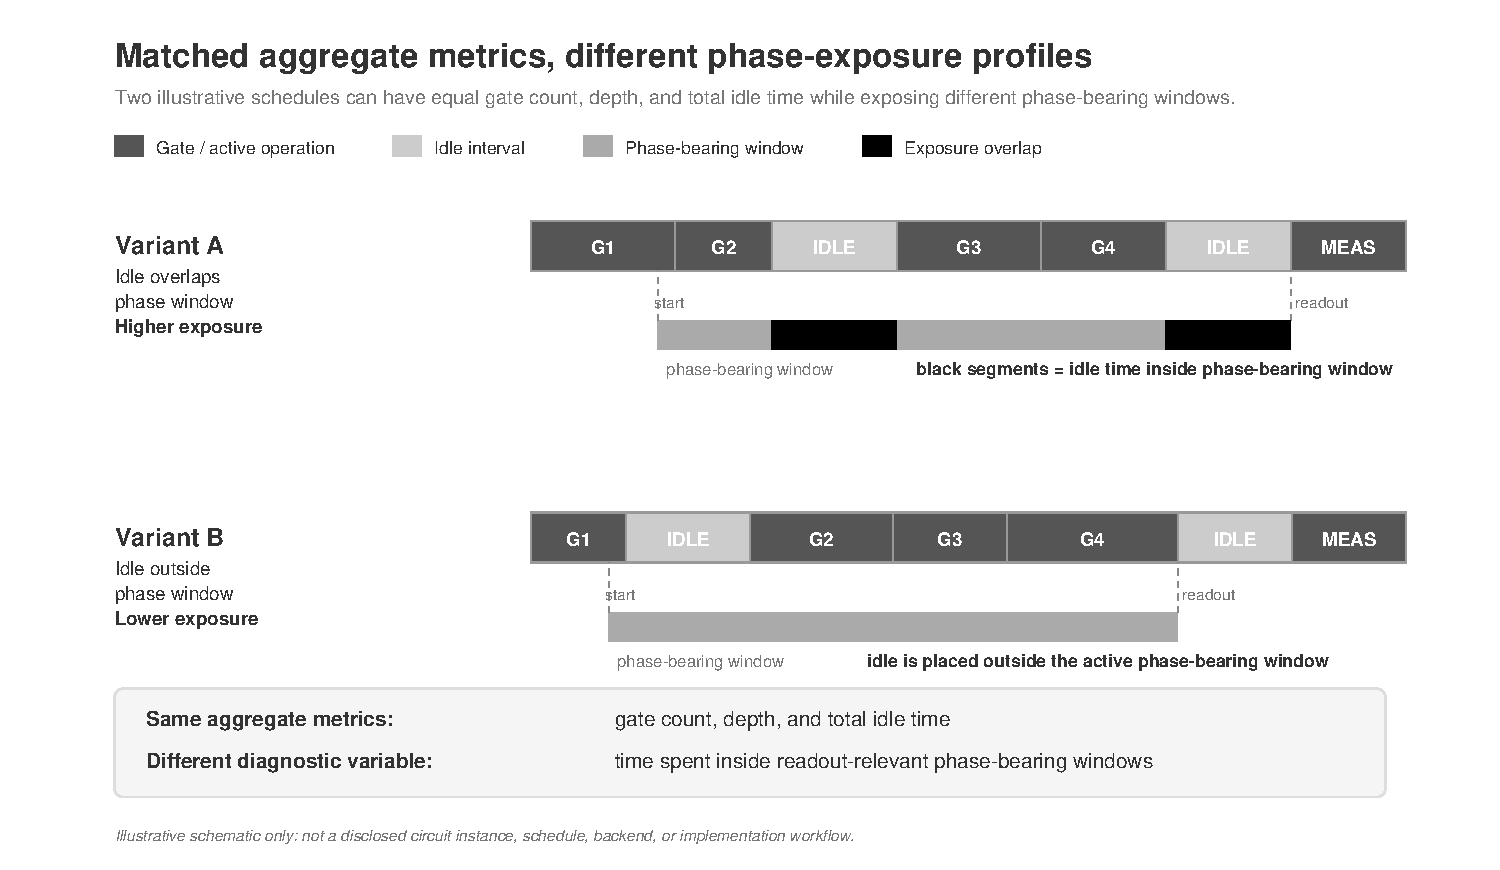
\includegraphics[width=0.95\textwidth]{figures/phase-exposure-schematic.pdf}
\caption{Schematic illustration of two schedules with identical aggregate metrics, including gate count, depth, and total idle time, but different phase-exposure profiles. Highlighted overlap regions indicate idle time inside readout-relevant phase-bearing windows. The figure is illustrative only and does not represent a disclosed circuit instance, schedule, backend, or implementation workflow.}
\label{fig:exposure-schematic}
\end{figure}

\section*{Hardware validation}

The phase-exposure hypothesis was validated on contemporary superconducting quantum hardware using families of logically equivalent or task-equivalent circuit variants. The variants were constructed to isolate execution-time exposure placement: where applicable, gate count, logical depth, total idle time, and hardware coherence parameters were held fixed or closely controlled, while the placement of idle intervals relative to phase-bearing execution windows was varied.

Across the tested validation families, the observed outcomes followed the phase-exposure prediction. Variants with greater idle exposure inside phase-bearing windows showed degraded measured outcomes relative to lower-exposure variants, even when aggregate metrics alone did not distinguish them.

Representative aggregate results from families of small-to-medium circuits, involving tens of qubits and thousands of shots per variant, are shown below. The table reports success proportions with Wilson 95\% confidence intervals, where success proportion denotes the fraction of shots yielding the expected readout for the circuit family.

\begin{center}
\renewcommand{\arraystretch}{1.25}
\begin{tabularx}{\textwidth}{>{\raggedright\arraybackslash}p{0.23\textwidth}
>{\raggedright\arraybackslash}p{0.34\textwidth}
>{\raggedright\arraybackslash}X}
\toprule
Validation family & Controlled contrast & Observed result \\
\midrule
Scheduling exposure &
Same logical work; exposure shifted by scheduling &
Lower-exposure variant: 0.942, Wilson 95\% CI [0.933, 0.950].

Higher-exposure variant: 0.435, Wilson 95\% CI [0.418, 0.453]. \\
\midrule
Idle-placement sensitivity &
Same inserted idle duration; idle placed before, split across, or after phase-bearing structure &
Late-idle variant: 0.790, Wilson 95\% CI [0.769, 0.810].

Split-idle variant: 0.401, Wilson 95\% CI [0.377, 0.426].

Early-idle variant: 0.297, Wilson 95\% CI [0.275, 0.321]. \\
\midrule
Per-qubit coherence exposure &
Same coherence-sensitive structure placed on different physical qubits &
Lower-risk placement: 0.639, Wilson 95\% CI [0.614, 0.663].

Higher-risk placement: 0.529, Wilson 95\% CI [0.503, 0.554]. \\
\bottomrule
\end{tabularx}
\end{center}

These results validate execution-time phase exposure as a real explanatory variable in circuit evaluation. The practical discovery is that coherence risk is not determined by total idle time alone. It depends on whether elapsed time overlaps phase-bearing quantum information relevant to the intended readout.

The underlying validation artifacts include real-hardware, offline/preflight, and ideal-control outputs. They are retained separately because the raw scheduled-execution reports and rendered diagnostic outputs are large. This whitepaper reports only sanitized aggregate validation results: no circuit definitions, job identifiers, report schemas, implementation details, or non-public workflow material are disclosed.

The specific techniques used to isolate, measure, and attribute execution-time phase exposure are the subject of a pending patent application and are not disclosed in this whitepaper.

\section*{From optimization by trial to exposure-aware diagnosis}

Today, many circuit-improvement workflows are necessarily heuristic. Engineers vary transpiler settings, routing choices, scheduling policies, decoupling sequences, and backend selections. Some variants perform better than others. The next challenge is to understand why.

Execution-time phase exposure offers a way to make those iterations more interpretable.

Instead of comparing variants only by gate count, depth, or total idle time, one can ask whether a variant has shifted exposure away from fragile phase-bearing windows, concentrated exposure on lower-risk qubits, or reduced the amount of time that entangled or phase-sensitive structure remains exposed.

That gives circuit optimization a more physically meaningful diagnostic target.

In this sense, the contribution is not just another metric. It is a change in what is being measured:
\[
\text{from aggregate scheduled time}
\quad\longrightarrow\quad
\text{readout-relevant phase exposure}.
\]

\section*{Implications}

Execution-time phase exposure suggests several practical directions for quantum engineering.

It can help explain why logically equivalent circuits behave differently after transpilation.

It can identify idle intervals that are likely more consequential than their duration alone suggests.

It can enable more interpretable A/B testing of transpiler and scheduler variants.

It can help prioritize where mitigation strategies such as scheduling changes or dynamical decoupling may matter most.

It offers a natural diagnostic target for future exposure-aware compilation and scheduling workflows.

It can provide a clearer diagnostic language for comparing circuit variants on noisy hardware.

It can help bridge the gap between hardware characterization and circuit-specific execution behavior.

Most importantly, it shifts attention from the presence of idle time to the role of idle time within the execution.

That distinction becomes more important as quantum processors scale. Wider devices and more complex circuits create increasingly uneven exposure profiles. Aggregate metrics become less able to explain performance. Exposure-aware diagnostics become more valuable.

\section*{Closing perspective}

Quantum hardware metrics will continue to improve. Transpilers, schedulers, calibration systems, and mitigation strategies will continue to become more sophisticated. But circuit performance will remain difficult to interpret if evaluation stops at aggregate quantities.

The central discovery is that coherence risk is not determined by total idle time alone. It depends on whether elapsed time overlaps phase-bearing quantum information relevant to the intended readout.

By reframing idle time as phase-bearing exposure, this diagnostic layer closes a long-standing explanatory gap between hardware characterization and circuit-specific outcomes. It shifts quantum engineering from purely aggregate metrics toward execution-time semantics.

Idle time is not the primitive.

Phase-bearing exposure is.

\end{document}
